\documentclass{beamer}
\usepackage{beamerthemesplit}
\usepackage{wrapfig}
\usetheme{SPbGU}
\usepackage{pdfpages}
\usepackage{amsmath}
\usepackage{cmap} 
\usepackage[T2A]{fontenc} 
\usepackage[utf8]{inputenc}
\usepackage[english,russian]{babel}
\usepackage{indentfirst}
\usepackage{amsmath}
\usepackage{tikz}
\usepackage{multirow}
\usepackage[noend]{algpseudocode}
\usepackage{algorithm}
\usepackage{algorithmicx}
\usepackage{listings}
\usetikzlibrary{shapes,arrows}
\usepackage{fancyvrb}
\newtheorem{rutheorem}{Теорема}
\newtheorem{ruproof}{Доказательство}
\newtheorem{rudefinition}{Определение}
\newtheorem{rulemma}{Лемма}

\beamertemplatenavigationsymbolsempty

\title[]{Синтаксический анализ контекстно-свободной аппроксимации}
\subtitle[]{}
% То, что в квадратных скобках, отображается в левом нижнем углу. 
\institute[]{}

% То, что в квадратных скобках, отображается в левом нижнем углу.
\author[Дмитрий Ковалев]{Дмитрий Ковалев}

\date{15 октября 2016г.}

\definecolor{orange}{RGB}{179,36,31}

\begin{document}
{

 %Лого университета или организации, отображается в шапке титульного листа
\begin{frame}
%	\begin{table}
%	\centering
%		\begin{tabular}{p{3cm} p{3cm} p{3cm}}
%			\begin{center}
%				{
\includegraphics[width=1.5cm]{pictures/jb.png}}
%			\end{center}
%			&
%		  \begin{center}
%		  	{
\includegraphics[width=1.5cm]{pictures/SPbGU_Logo.png}}
%		  \end{center}
%		  &
%		  \begin{center}
%		  	{
\includegraphics[width=1.5cm]{pictures/yacc.pdf}}
%		  \end{center}
%		\end{tabular}
%	\end{table}
\begin{center}
	{
\includegraphics[width=1.5cm]{pictures/SPbGU_Logo.png}}
\end{center}
\titlepage
\end{frame}
}

%\maketitle

\begin{frame}[fragile]
	\transwipe[direction=90]
	\frametitle{Динамически формируемый код}  
	\begin{itemize}
		\item SQL-запросы в C$\#$    
			\begin{Verbatim}[commandchars=\\\{\}]
  \textcolor{blue}{private void} Example (\textcolor{blue}{int} cond) \{
      \textcolor{blue}{string} columnName = cond > \textcolor{gray}{42} ? \textcolor{red}{"X"} : \textcolor{red}{"Y"};
      \textcolor{blue}{string} queryString = 
          \textcolor{red}{"SELECT name"} + columnName + \textcolor{red}{" FROM table"};
      Program.ExecuteImmediate(queryString);
  \}
				\end{Verbatim}
		\pause
		\item Генерация HTML-страниц в PHP
			\begin{Verbatim}[commandchars=\\\{\}]	
  <?php 
      \$name = \textcolor{red}{'your name'};
      echo \textcolor{red}{'<table>} 
           \textcolor{red}{<tr><th>Name</th></tr>}  
           \textcolor{red}{<tr><td>'}.\$name.\textcolor{red}{'</td></tr>} 
           \textcolor{red}{</table>'};
  ?>
			\end{Verbatim}
	\end{itemize}
\end{frame}

\begin{frame}[fragile]
	\transwipe[direction=90]
	\frametitle{Существующие решения} 
		\begin{table}[h]
			\centering
			\begin{tabular}{p{4.6cm} p{4.6cm}}
				\begin{center}
					\begin{Verbatim}[commandchars=\\\{\}]
x = \textcolor{red}{"a"}
while ...
    x = \textcolor{red}{"["} . x . \textcolor{red}{"]"}
print x
					\end{Verbatim}
				\end{center}
				&
				\begin{center}
					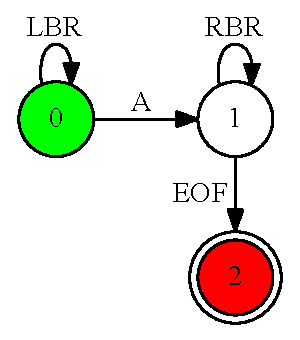
\includegraphics[width=2.5cm]{pictures/reg_app.pdf}	
				\end{center}	  		
			\end{tabular}
		\end{table}
		\begin{itemize}
			\item Java String Analyzer, Alvor, PHP String Analyzer
			\begin{itemize}
				\item Регулярная/КС-аппроксимация
				\item Не строят структурного представления кода
			\end{itemize}
		\end{itemize}
\end{frame}

\begin{frame}[fragile]
	\transwipe[direction=90]
	\frametitle{Абстрактный синтаксический анализ}
	\begin{table}[h]
	\centering
	\begin{tabular}{p{4.3cm} p{3cm} p{3cm}}
		\begin{center}
			\begin{Verbatim}[commandchars=\\\{\}]
x = \textcolor{red}{"a"}
while ...
    x = \textcolor{red}{"["} . x . \textcolor{red}{"]"}
print x
			\end{Verbatim}
		\end{center}
		&
		\begin{center}
			\begin{Verbatim}[commandchars=\\\{\},  
			codes={\catcode`$=3}]
X0 = \textcolor{red}{a} 
X1 = X0 $\cup$ X2
X2 = \textcolor{red}{[} . X1 . \textcolor{red}{]}
X3 = X1 
			\end{Verbatim}
		\end{center}
		&
		\begin{center}
			\begin{Verbatim}[commandchars=\\\{\}]
X0 ::= \textcolor{red}{a}
X1 ::= X0 | X2
X2 ::= \textcolor{red}{[} X1 \textcolor{red}{]} 
X3 ::= X1
			\end{Verbatim}
		\end{center}
	\end{tabular}
	\end{table}
	\begin{itemize}
		\item Kyung-Goo Doh, Hyunha Kim, David A. Schmidt ``Abstract LR-parsing'', 2011
		\item Решение dataflow-уравнений (LFP) в домене LR-стеков 
		\item Отсутствует структурное представление результатов
		\item КС-аппроксимация
	\end{itemize}
\end{frame}

\begin{frame}[fragile]
	\transwipe[direction=90]
	\frametitle{YaccConstructor}
	\begin{itemize}
		\item Анализ регулярной аппроксимации на основе алгоритма Generalized LL (Анастасия Рагозина, 2016)
	\end{itemize}
		\begin{table}[h]
			\centering
			\begin{tabular}{p{4cm} p{6cm}}
				\begin{minipage}{3in}
					\begin{Verbatim}[commandchars=\\\{\}]
x = \textcolor{red}{"a"}
while ...
    x = \textcolor{red}{"["} . x . \textcolor{red}{"]"}
print x
					\end{Verbatim}
				\end{minipage}
				&
				\begin{center}
					\multirow{-4}*{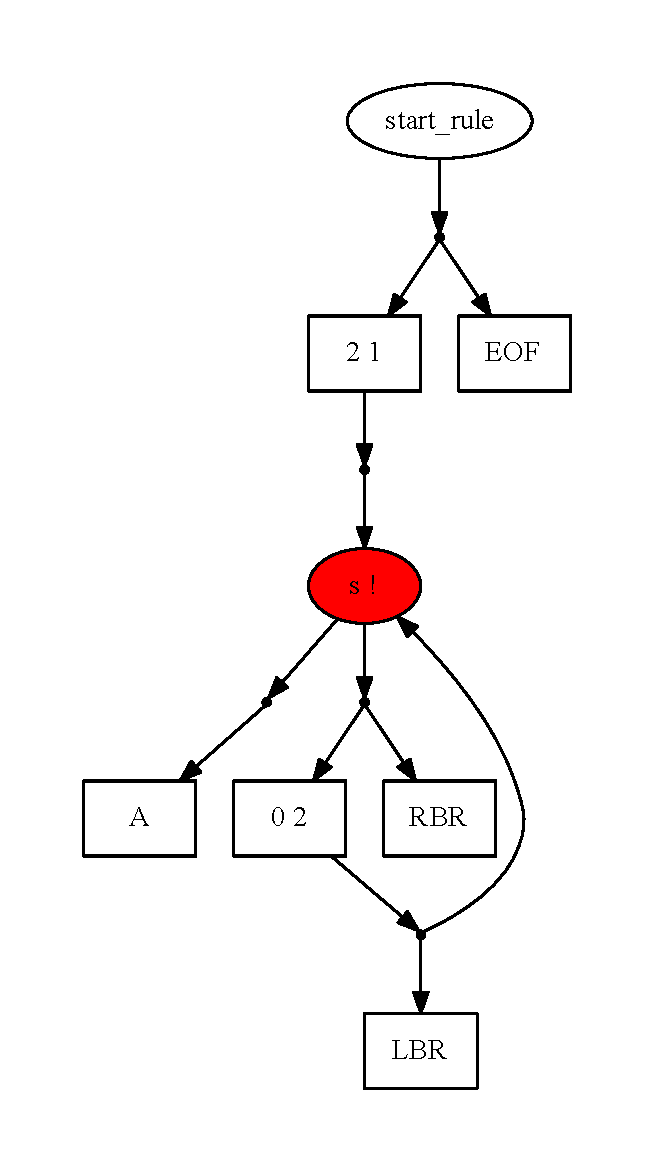
\includegraphics[width=4cm]{pictures/sppf.pdf}}
				\end{center}
				\\
				\vspace{-10pt}
				\begin{center}
					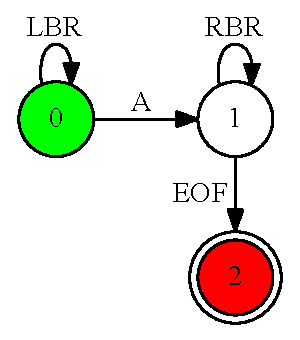
\includegraphics[width=2cm]{pictures/reg_app.pdf}	
				\end{center}
				&
				\\
				\vspace{-20pt}
				$$
					\begin{array}{crcl}
						&start &::=& s \\
						&s & ::= & \mbox{\texttt{LBR }} s \mbox{\texttt{ RBR }} | \ \mbox{\texttt{A}}\\
					\end{array}
				$$
			\end{tabular}
		\end{table}
\end{frame}


\begin{frame}
	\transwipe[direction=90]
	\frametitle{Generalized LL (GLL)}
	\begin{itemize}
		\item Работает с произвольными КС-грамматиками
		\item Стандартные LL(k)-таблицы, допускаются конфликты в ячейках
		\pause
		\item Дескриптор --- $(L, u, i, w)$, где
		\begin{itemize}
			\item $L$ --- позиция в грамматике вида $A \rightarrow \alpha \cdot X \beta$
			\item $u$ --- вершина стека
			\item $i$ --- позиция во входном потоке
			\item $w$ --- узел SPPF
		\end{itemize}
		\pause
		\item В случае конфликта создаются дескрипторы для каждого правила в ячейке таблицы
		\pause
		\item В процессе анализа поддерживаются очередь обработки и мн-во созданных ранее дескрипторов		
	\end{itemize}
\end{frame}

\begin{frame}[fragile]
	\transwipe[direction=90]
	\frametitle{Модификация GLL}
	\begin{itemize}
		\item Вход --- детерминированный конечный автомат
		\item Вместо позиции в строке --- номер вершины автомата
		\pause
		\item Для текущей вершины просматриваются все исходящие ребра
	\end{itemize}
	\begin{table}
		\begin{tabular}{p{5cm} p{5cm}}
			$$
				\begin{array}{crcl}
					&start &::=& s \\
					&s & ::= & \cdot \ \mbox{\texttt{LBR }} s \mbox{\texttt{ RBR }} \\
					&s & ::= & \mbox{\texttt{A}}\\
				\end{array}
			$$
			&
			\begin{center}
				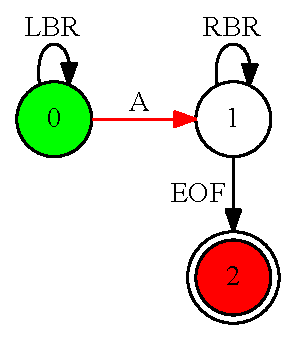
\includegraphics[width=3cm]{pictures/reg_app_error.pdf}
			\end{center}
		\end{tabular}
	\end{table}
	$$\text{Некорректные строки, генерируемые автоматом}: ``[A``,\ ``[[A``,\ ``[A]]`` ,\ ...$$
\end{frame}

\begin{frame}[fragile]
	\transwipe[direction=90]
	\frametitle{GLL \& КС-аппроксимация}
	\begin{table}
		\begin{tabular}{p{5cm} p{5cm}}
			\begin{center}
				\begin{Verbatim}[commandchars=\\\{\}]
x = \textcolor{red}{"a"}
while ...
    x = \textcolor{red}{"["} . x . \textcolor{red}{"]"}
print x
				\end{Verbatim}
			\end{center}
		&
			\begin{center}
				\begin{Verbatim}[commandchars=\\\{\}]
X0 ::= \textcolor{red}{a}
X1 ::= X0 | X2
X2 ::= \textcolor{red}{[} X1 \textcolor{red}{]} 
X3 ::= X1
				\end{Verbatim}
			\end{center}
		\end{tabular}
	\end{table}
	\begin{itemize}
		\item Необходимо представление аппроксимирующей грамматики, подходящее для GLL
	\end{itemize}
\end{frame}

\begin{frame}
	\transwipe[direction=90]
	\frametitle{Постановка задачи}
	\textbf{Целью} работы является повышение точности диагностики ошибок в динамически формируемом коде (в рамках YC)
	
	\textbf{Задачи}:
	\begin{itemize}
		\item Найти подходящее представление КС-аппроксимации
		\item Адаптировать GLL для работы с таким представлением
	\end{itemize}
\end{frame}

%\begin{frame}[fragile]
%	\transwipe[direction=90]
%	\frametitle{Абстрактный анализ}
%
%	\begin{table}[h]
%		\centering
%		\begin{tabular}{p{4.5cm} p{3cm} p{3cm}}
%			\begin{center}
%				\begin{Verbatim}[commandchars=\\\{\}]
%x = \textcolor{red}{"a"}
%while ...
%    x = \textcolor{red}{"["} . x . \textcolor{red}{"]"}
%print x
%				\end{Verbatim}
%			\end{center}
%			&
%			\begin{center}
%				\begin{Verbatim}[commandchars=\\\{\}, codes={\catcode`$=3}]
%X0 = \textcolor{red}{a} 
%X1 = X0 $\cup$ X2
%X2 = \textcolor{red}{[} . X1 . \textcolor{red}{]}
%X3 = X1 
%				\end{Verbatim}
%			\end{center}
%			&
%			\pause
%			\begin{center}
%				\begin{Verbatim}[commandchars=\\\{\}]
%X0 ::= \textcolor{red}{a}
%X1 ::= X0 | X2
%X2 ::= \textcolor{red}{[} X1 \textcolor{red}{]} 
%X3 ::= X1
%				\end{Verbatim}
%			\end{center}	
%		\end{tabular}
%	\end{table}
%
%	\pause
%	\begin{itemize}
%		\item Необходимо представление получившейся КС-грамматики, подходящее для GLL-анализа
%	\end{itemize}
%\end{frame}

\begin{frame}[fragile]
	\transwipe[direction=90]
	\frametitle{Замечание}
	\begin{table}
	\centering
		\begin{tabular}{p{3cm} p{0.5cm} p{3cm} p{0.5cm} p{3cm}}
				\vspace{5pt}
				\begin{Verbatim}[commandchars=\\\{\}]
X0 ::= \textcolor{red}{a}
X1 ::= X0 | X2
X2 ::= \textcolor{red}{[} X1 \textcolor{red}{]} 
X3 ::= X1
				\end{Verbatim}
				&
				\pause
				$$\Huge {\sim}$$
				&
				\vspace{10pt}
				\begin{Verbatim}[commandchars=\\\{\}]
X1 ::= \textcolor{red}{a} | X2
X2 ::= \textcolor{red}{[} X1 \textcolor{red}{]} 
X3 ::= X1
				\end{Verbatim}
				&
				\pause
				$$\Huge{\sim}$$
				&
				\vspace{10pt}
				\begin{Verbatim}[commandchars=\\\{\}]
X1 ::= \textcolor{red}{a}
X1 ::= \textcolor{red}{[} X1 \textcolor{red}{]} 
X3 ::= X1
				\end{Verbatim}
		\end{tabular}
	\end{table}
\end{frame}

\begin{frame}[fragile]
	\transwipe[direction=90]
	\frametitle{Grammar Flow Graph (GFG)}
	\begin{table}
	\centering
		\begin{tabular}{p{4cm} p{8cm}}
			\begin{center}
				\begin{BVerbatim}[commandchars=\\\{\}]
X3 ::= X1
X1 ::= \textcolor{red}{[} X1 \textcolor{red}{]}
X1 ::= \textcolor{red}{a} 
					\end{BVerbatim}
			\end{center}
				&
				\begin{center}
					\hspace{20pt} \multirow{-3}*{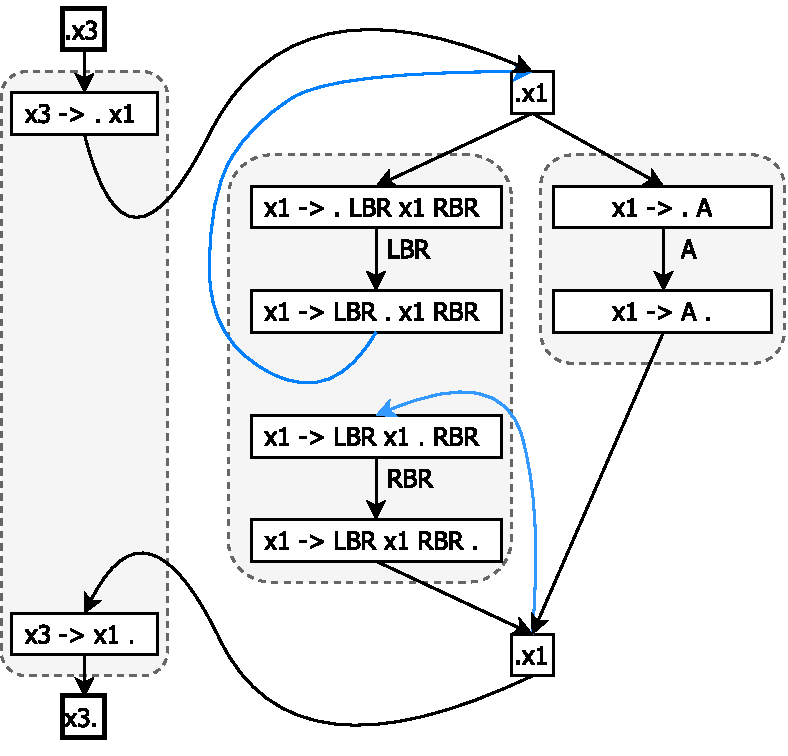
\includegraphics[width=6cm]{pictures/GFG2.pdf}}
				\end{center}
				\\
				\begin{table}
				\centering
					\begin{tabular}{p{1.8cm} | p{1.8cm}}
						{\small $A \rightarrow \alpha \cdot X \beta$}
						&
						{\small call node}
						\\ \hline
						{\small $A \rightarrow \alpha X \cdot \beta$}
						&
						{\small return node}
					\end{tabular}
				\end{table}
		\end{tabular}
	\end{table}
	\begin{itemize}
		\item Keshav Pingali, Gianfranco Bilardi ``A Graphical Model for Context-Free Grammar Parsing'', 2015
	\end{itemize}
\end{frame}

\begin{frame}
	\transwipe[direction=90]
	\frametitle{GLL \& GFG}
	\begin{itemize}
%		\item Дескрипторы имеют вид $(L, u, i, w, v)$, где $v$ --- вершина CR-стека
		\item В случае недетерминированного выбора создается дескриптор для каждого пути
			\begin{center}
				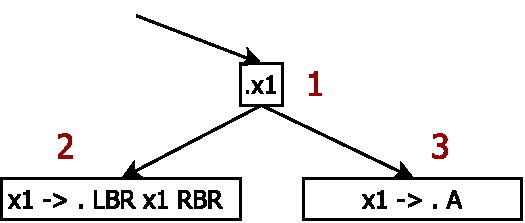
\includegraphics[width=5cm]{pictures/fork.pdf}
				\vspace{10pt}
				
				Current : $(L, u, 1, w)$
				
				AddToQueue \ $(L, u, 2, w) \ (L, u, 3, w)$
			\end{center}
	\end{itemize}
\end{frame}

\begin{frame}
	\transwipe[direction=90]
	\frametitle{GLL \& GFG}
	\begin{itemize}
		\item Необходимо поддерживать CR-стек		
	\end{itemize}
	\begin{table}
	\centering
		\begin{tabular}{p{6cm} p{4cm}}
			\begin{center}
				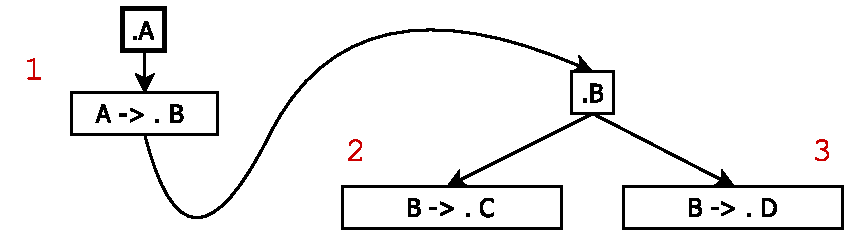
\includegraphics[width=6cm]{pictures/stack_fork.pdf}
			\end{center}
			&
			\begin{center}
				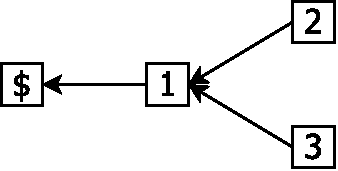
\includegraphics[width=3cm]{pictures/CR_gss.pdf}
			\end{center}
		\end{tabular}
	\end{table}
	\begin{itemize}
		\item Graph-structured stack (GSS)
		\item Дескрипторы имеют вид $(L, u, i, w, v)$, где $v$ --- вершина CR-стека
	\end{itemize}
\end{frame}

\begin{frame}[fragile]
	\transwipe[direction=90]
	\frametitle{Эксперименты}
	\begin{table}
	\centering
		\begin{tabular}{p{5cm} p{5cm}}
			\begin{Verbatim}[commandchars=\\\{\}]
x = \textcolor{red}{"a"}
while ...
    x = \textcolor{red}{"["} . x . \textcolor{red}{"]"}
print x
			\end{Verbatim}
			&
			\begin{table}
				\centering
				\begin{tabular}{p{2.5cm} | c}
					Аппроксимация & Кол-во ошибок \\ \hline
					Регулярная & 5 \\ \hline
					КС (GFG) & 0
				\end{tabular}
			\end{table}
		\end{tabular}
	\end{table}
\end{frame}

\begin{frame}
	\transwipe[direction=90]
	\frametitle{Результаты}
	\begin{itemize}
		\item Реализовано преобразование грамматики в GFG
		\item GLL адаптирован для работы с GFG
	\end{itemize}
\end{frame}

\end{document}
